% Generated by julia/scripts/generate_manuscript_numerical_artifacts.jl.
% Source: experiments/results/summaries/canonical_model_convergence.csv.
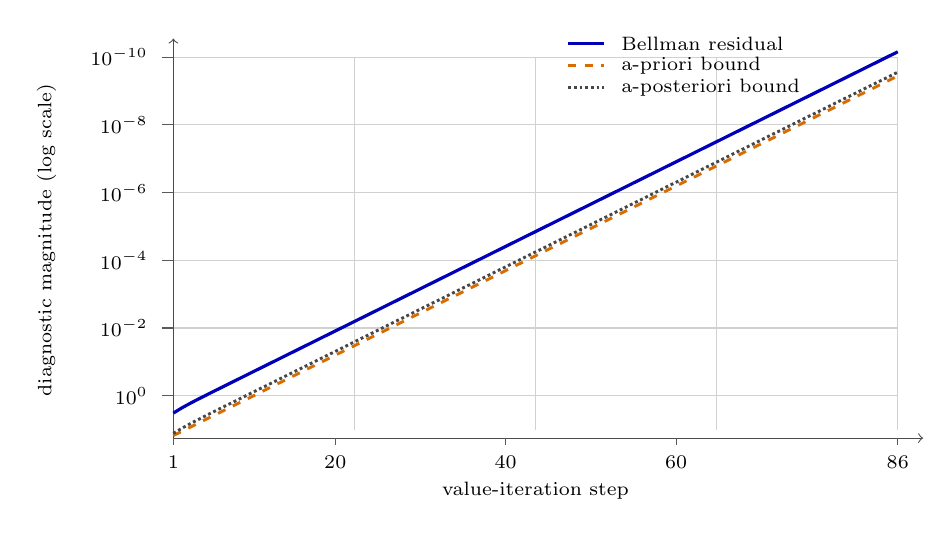
\begin{tikzpicture}[x=0.92cm,y=0.43cm,font=\scriptsize]
  \draw[black!18] (0,-1) grid[xstep=2.5,ystep=2] (10,10);
  \draw[->,black!70] (0,-1.25) -- (10.35,-1.25);
  \draw[->,black!70] (0,-1.25) -- (0,10.55);
  \foreach \x/\label in {0/1,2.235/20,4.588/40,6.941/60,10/86} {
    \draw[black!65] (\x,-1.25) -- (\x,-1.45);
    \node[anchor=north] at (\x,-1.5) {\label};
  }
  \foreach \y/\label in {0/{$10^{0}$},2/{$10^{-2}$},4/{$10^{-4}$},6/{$10^{-6}$},8/{$10^{-8}$},10/{$10^{-10}$}} {
    \draw[black!65] (0,\y) -- (-0.16,\y);
    \node[anchor=east] at (-0.22,\y) {\label};
  }
  \draw[blue!72!black,line width=1.15pt] (0.0,-0.511883) -- (0.117647,-0.358173) -- (0.235294,-0.22066) -- (0.352941,-0.090372) -- (0.470588,0.036815) -- (0.588235,0.162694) -- (0.705882,0.288025) -- (0.823529,0.413127) -- (0.941176,0.538134) -- (1.058824,0.663101) -- (1.176471,0.788052) -- (1.294118,0.912996) -- (1.411765,1.037936) -- (1.529412,1.162876) -- (1.647059,1.287815) -- (1.764706,1.412754) -- (1.882353,1.537693) -- (2.0,1.662632) -- (2.117647,1.78757) -- (2.235294,1.912509) -- (2.352941,2.037448) -- (2.470588,2.162386) -- (2.588235,2.287325) -- (2.705882,2.412264) -- (2.823529,2.537203) -- (2.941176,2.662141) -- (3.058824,2.78708) -- (3.176471,2.912019) -- (3.294118,3.036958) -- (3.411765,3.161896) -- (3.529412,3.286835) -- (3.647059,3.411774) -- (3.764706,3.536713) -- (3.882353,3.661651) -- (4.0,3.78659) -- (4.117647,3.911529) -- (4.235294,4.036468) -- (4.352941,4.161406) -- (4.470588,4.286345) -- (4.588235,4.411284) -- (4.705882,4.536222) -- (4.823529,4.661161) -- (4.941176,4.7861) -- (5.058824,4.911039) -- (5.176471,5.035977) -- (5.294118,5.160916) -- (5.411765,5.285855) -- (5.529412,5.410794) -- (5.647059,5.535732) -- (5.764706,5.660671) -- (5.882353,5.78561) -- (6.0,5.910549) -- (6.117647,6.035487) -- (6.235294,6.160426) -- (6.352941,6.285365) -- (6.470588,6.410304) -- (6.588235,6.535242) -- (6.705882,6.660181) -- (6.823529,6.78512) -- (6.941176,6.910058) -- (7.058824,7.034997) -- (7.176471,7.159936) -- (7.294118,7.284875) -- (7.411765,7.409813) -- (7.529412,7.534752) -- (7.647059,7.659691) -- (7.764706,7.78463) -- (7.882353,7.909568) -- (8.0,8.034507) -- (8.117647,8.159446) -- (8.235294,8.284384) -- (8.352941,8.409323) -- (8.470588,8.534262) -- (8.588235,8.6592) -- (8.705882,8.784139) -- (8.823529,8.909078) -- (8.941176,9.034016) -- (9.058824,9.158954) -- (9.176471,9.283893) -- (9.294118,9.408832) -- (9.411765,9.533771) -- (9.529412,9.658708) -- (9.647059,9.783648) -- (9.764706,9.908585) -- (9.882353,10.033524) -- (10.0,10.15846);
  \draw[orange!85!black,line width=1.05pt,dashed] (0.0,-1.176091) -- (0.117647,-1.051153) -- (0.235294,-0.926214) -- (0.352941,-0.801275) -- (0.470588,-0.676336) -- (0.588235,-0.551398) -- (0.705882,-0.426459) -- (0.823529,-0.30152) -- (0.941176,-0.176581) -- (1.058824,-0.051643) -- (1.176471,0.073296) -- (1.294118,0.198235) -- (1.411765,0.323174) -- (1.529412,0.448112) -- (1.647059,0.573051) -- (1.764706,0.69799) -- (1.882353,0.822929) -- (2.0,0.947867) -- (2.117647,1.072806) -- (2.235294,1.197745) -- (2.352941,1.322683) -- (2.470588,1.447622) -- (2.588235,1.572561) -- (2.705882,1.6975) -- (2.823529,1.822438) -- (2.941176,1.947377) -- (3.058824,2.072316) -- (3.176471,2.197255) -- (3.294118,2.322193) -- (3.411765,2.447132) -- (3.529412,2.572071) -- (3.647059,2.69701) -- (3.764706,2.821948) -- (3.882353,2.946887) -- (4.0,3.071826) -- (4.117647,3.196765) -- (4.235294,3.321703) -- (4.352941,3.446642) -- (4.470588,3.571581) -- (4.588235,3.696519) -- (4.705882,3.821458) -- (4.823529,3.946397) -- (4.941176,4.071336) -- (5.058824,4.196274) -- (5.176471,4.321213) -- (5.294118,4.446152) -- (5.411765,4.571091) -- (5.529412,4.696029) -- (5.647059,4.820968) -- (5.764706,4.945907) -- (5.882353,5.070846) -- (6.0,5.195784) -- (6.117647,5.320723) -- (6.235294,5.445662) -- (6.352941,5.570601) -- (6.470588,5.695539) -- (6.588235,5.820478) -- (6.705882,5.945417) -- (6.823529,6.070355) -- (6.941176,6.195294) -- (7.058824,6.320233) -- (7.176471,6.445172) -- (7.294118,6.57011) -- (7.411765,6.695049) -- (7.529412,6.819988) -- (7.647059,6.944927) -- (7.764706,7.069865) -- (7.882353,7.194804) -- (8.0,7.319743) -- (8.117647,7.444682) -- (8.235294,7.56962) -- (8.352941,7.694559) -- (8.470588,7.819498) -- (8.588235,7.944437) -- (8.705882,8.069375) -- (8.823529,8.194314) -- (8.941176,8.319253) -- (9.058824,8.444191) -- (9.176471,8.56913) -- (9.294118,8.694069) -- (9.411765,8.819008) -- (9.529412,8.943946) -- (9.647059,9.068885) -- (9.764706,9.193824) -- (9.882353,9.318763) -- (10.0,9.443701);
  \draw[black!72,line width=1.05pt,densely dotted] (0.0,-1.113943) -- (0.117647,-0.960233) -- (0.235294,-0.82272) -- (0.352941,-0.692432) -- (0.470588,-0.565245) -- (0.588235,-0.439366) -- (0.705882,-0.314035) -- (0.823529,-0.188933) -- (0.941176,-0.063926) -- (1.058824,0.061041) -- (1.176471,0.185992) -- (1.294118,0.310936) -- (1.411765,0.435876) -- (1.529412,0.560816) -- (1.647059,0.685755) -- (1.764706,0.810694) -- (1.882353,0.935633) -- (2.0,1.060572) -- (2.117647,1.18551) -- (2.235294,1.310449) -- (2.352941,1.435388) -- (2.470588,1.560326) -- (2.588235,1.685265) -- (2.705882,1.810204) -- (2.823529,1.935143) -- (2.941176,2.060081) -- (3.058824,2.18502) -- (3.176471,2.309959) -- (3.294118,2.434898) -- (3.411765,2.559836) -- (3.529412,2.684775) -- (3.647059,2.809714) -- (3.764706,2.934653) -- (3.882353,3.059591) -- (4.0,3.18453) -- (4.117647,3.309469) -- (4.235294,3.434408) -- (4.352941,3.559346) -- (4.470588,3.684285) -- (4.588235,3.809224) -- (4.705882,3.934162) -- (4.823529,4.059101) -- (4.941176,4.18404) -- (5.058824,4.308979) -- (5.176471,4.433917) -- (5.294118,4.558856) -- (5.411765,4.683795) -- (5.529412,4.808734) -- (5.647059,4.933672) -- (5.764706,5.058611) -- (5.882353,5.18355) -- (6.0,5.308489) -- (6.117647,5.433427) -- (6.235294,5.558366) -- (6.352941,5.683305) -- (6.470588,5.808244) -- (6.588235,5.933182) -- (6.705882,6.058121) -- (6.823529,6.18306) -- (6.941176,6.307998) -- (7.058824,6.432937) -- (7.176471,6.557876) -- (7.294118,6.682815) -- (7.411765,6.807753) -- (7.529412,6.932692) -- (7.647059,7.057631) -- (7.764706,7.18257) -- (7.882353,7.307508) -- (8.0,7.432447) -- (8.117647,7.557386) -- (8.235294,7.682324) -- (8.352941,7.807263) -- (8.470588,7.932202) -- (8.588235,8.05714) -- (8.705882,8.182079) -- (8.823529,8.307018) -- (8.941176,8.431956) -- (9.058824,8.556894) -- (9.176471,8.681833) -- (9.294118,8.806772) -- (9.411765,8.931711) -- (9.529412,9.056648) -- (9.647059,9.181588) -- (9.764706,9.306525) -- (9.882353,9.431464) -- (10.0,9.5564);
  \draw[blue!72!black,line width=1.15pt] (5.45,10.4) -- (5.95,10.4);
  \node[anchor=west] at (6.05,10.4) {Bellman residual};
  \draw[orange!85!black,line width=1.05pt,dashed] (5.45,9.75) -- (5.95,9.75);
  \node[anchor=west] at (6.05,9.75) {a-priori bound};
  \draw[black!72,line width=1.05pt,densely dotted] (5.45,9.1) -- (5.95,9.1);
  \node[anchor=west] at (6.05,9.1) {a-posteriori bound};
  \node[anchor=north] at (5,-2.25) {value-iteration step};
  \node[rotate=90] at (-1.75,4.6) {diagnostic magnitude (log scale)};
\end{tikzpicture}
